%\section{Measurements with CC $\nu_{\mu}$ candidates \label{sec:nuprism_numu}}

\section{Combinations of off-axis neutrino spectra }
\label{sec:combos}

% Need to somehow also talk about NC here too.

As discussed in the previous section, $\nu$PRISM can reconstruct large, pure samples of charged current
events with a muon candidate and no other particles above Cherenkov threshold.  For each event, the
off-axis angle $\theta_{OA}$ is reconstructed and this observable implies additional information about the
distribution of possible neutrino energies based on the prior flux model.  Data binned in $\theta_{OA}$ and the
usual muon observables of momentum (or kinetic energy) and scattering angle are used to constrain the
cross section model.  In the typical approach, the data may be unfolded to find the cross-section in the
true variable of neutrino energy, muon momentum  and muon scattering angle.  However, unfolding relies 
on regularization to deal with the ill-defined nature of the problem, and may not perform well when 
unfolding for $\theta_{OA}$ to the neutrino energy.

We take an alternative approach of using the off-axis neutrino spectra impinging on $\nu$PRISM as a set of basis
functions.  We then write a spectrum of interest as a linear combination of the off-axis spectra:
\begin{equation}
F_{\nu_{\mu}}(E_{\nu}) = \sum_{i} c_{i}\phi^{i}_{\nu_{\mu}}(E_{\nu}).
\end{equation}
Here $F_{\nu_{\mu}}(E_{\nu})$ is an arbitrary function of interest, $\phi^{i}_{\nu_{\mu}}(E_{\nu})$ is the predicted spectrum
in the $i^{th}$ off-axis angle bin and $c_{i}$ are simply coefficients.  The challenge is to find a set of $c_{i}$
that approximately satisfy the equation while minimizing the statistical and systematic uncertainties that are propagated through the
linear combination.  Once the $c_{i}$ are found, we can write a similar equation for the observables:
\begin{equation}
N(p_{\mu},\theta_{\mu}|F_{\nu_{\mu}}(E_{\nu})) = \sum_{i} c_{i}N^{i}(p_{\mu},\theta_{\mu}).
\end{equation}
In this way, the final state particle multiplicities and kinematics can be measured for an given choice of 
of the input neutrino energy spectrum.  

The consequence of the nuPRISM flux combinations are that we can generate any neutrino flux shape within the kinematics specified by the detector position and beam line. Two immediate applications are evident: pseudo-monoenergetic neutrino beams for measurements of neutrino interactions on water, discussed in Section~\ref{sec:mono}, and neutrino fluxes which correspond to a set of standard (or non-standard) oscillation parameters (Section XXX)

\subsection{Pseudo-monoenergetic neutrino flux measurements}
\label{sec:mono}

% Neutrino vs. electron scattering.
%% Relevant variables of eA

While neutrinos are a unique probe of the axial structure of the nucleus, it has been challenging so-far to use measurements of neutrinos on nuclei. The canonical probe of nuclear structure is to scatter an electron of a known energy off a nuclear target. A comparison between the incident and recoil electron determines the energy transfer ($\omega$) and momentum transfer ($q^2$). Electron scattering experiments determine the electromagnetic structure of nuclei, quantified by the vector form factors; neutrino scattering experiments determine the axial form factors. One can infer the single nucleon form factors from scattering off of hydrogen and deuterium, and scattering off of different target materials determines the nuclear dependance.  The first critical difference between electron and neutrino scattering is that, unlike electron scattering, the incident neutrino energy is not well known, and measurements are therefore presented as averaged over the flux. In the case of QE, this results in multiple processes (single pion resonance production, multi-nucleon knockout) contributing ``QE'' measurements and complicates any  determination of how nuclear effects modify the QE cross section; in electron scattering, the kinematics alone determine QE interactions.  
%Additional information about the QE cross section can be inferred by comparing measurements made at different average neutrino beam energies, but this has not resulted in a coherent picture.
% cite what here.

With the nuPRISM technique, it will be possible to make cross section measurements of neutrinos on water which correspond to that which would be measured with a pseudo-monochromatic neutrino beam. Figure~\ref{fig:mono_beam} shows spectra generated with nuPRISM, shown with uncertainties on the predicted neutrino flux, and statistical combination included. Mono-chromatic beams can be constructed for any energy between {\color{red} XXXX and XXXX }, with approximately 15\% $\Delta E / E$.

\begin{figure}[htpb]
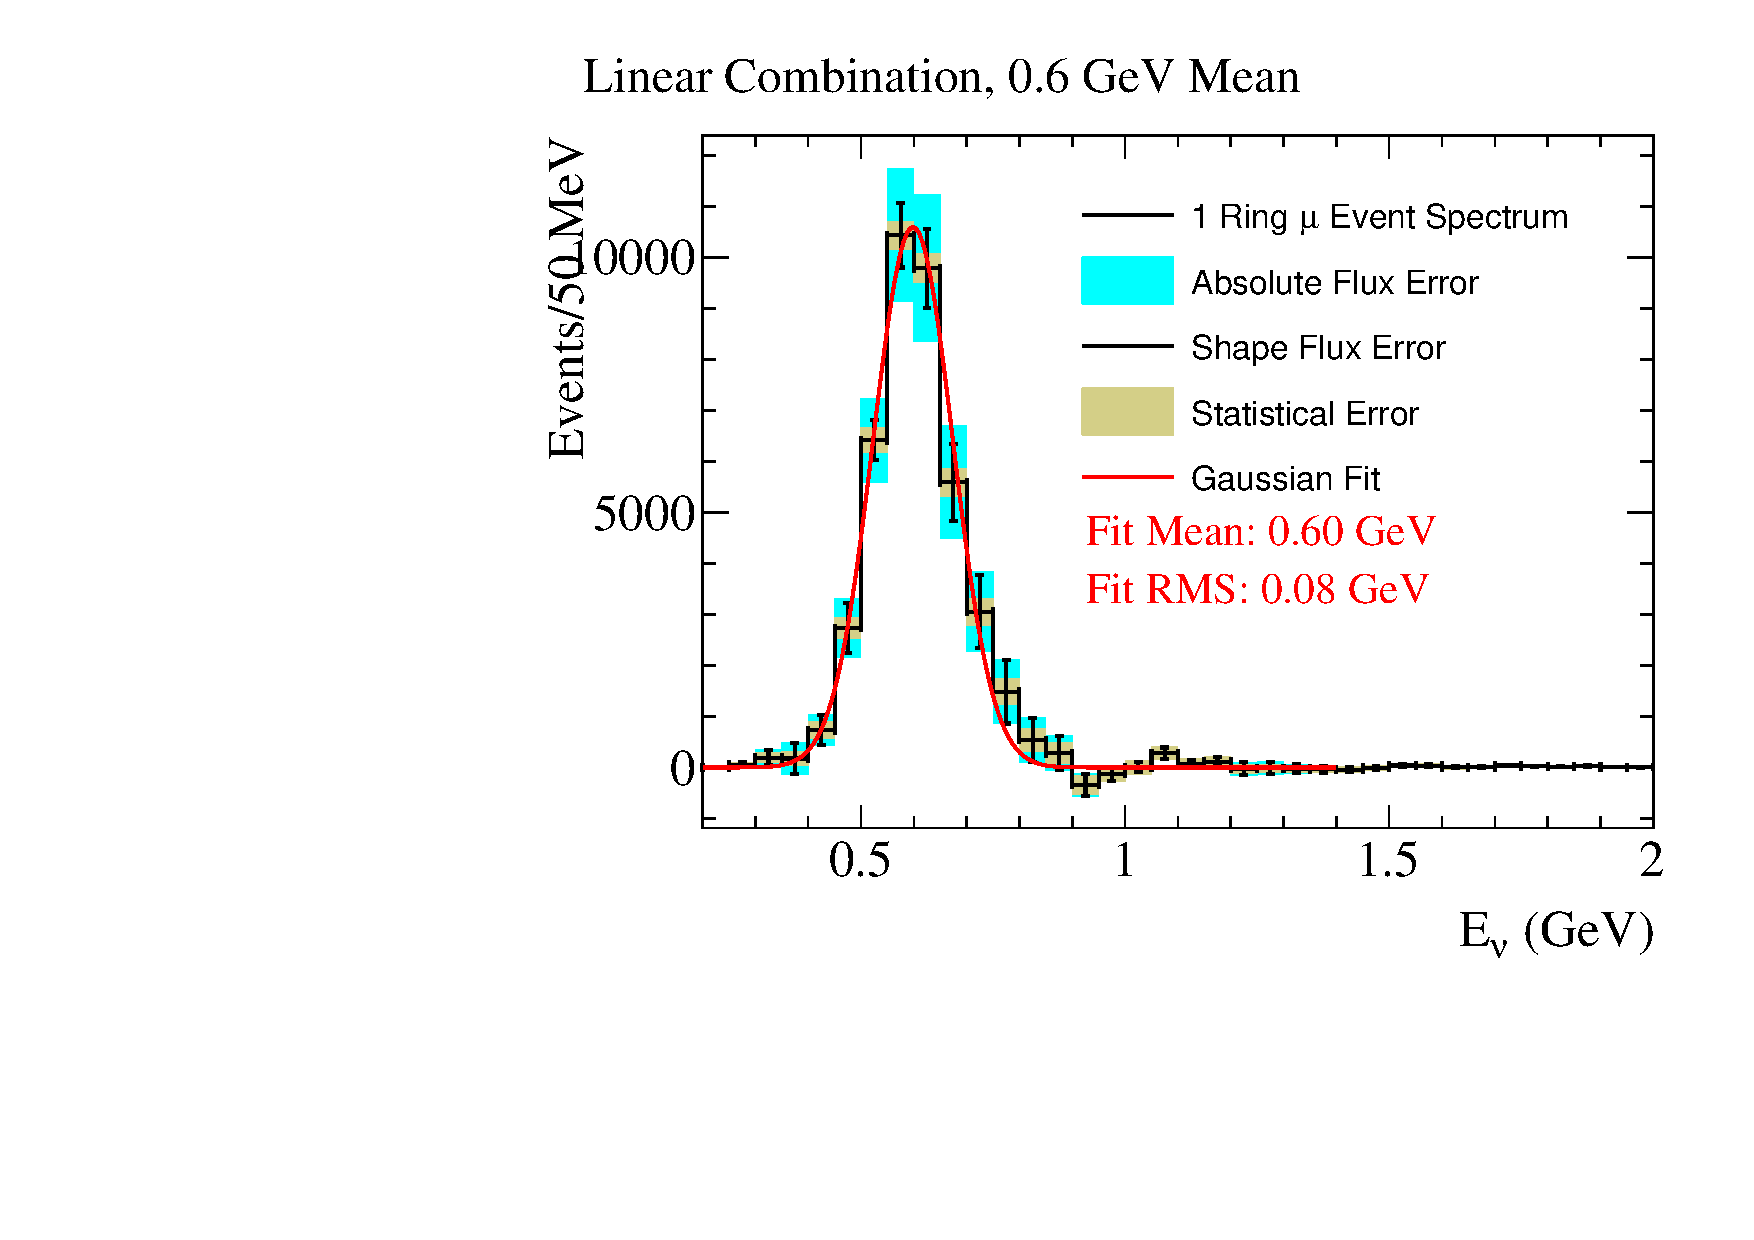
\includegraphics[width=0.45\textwidth]{figures/lc_etrue_600mev.pdf} \\
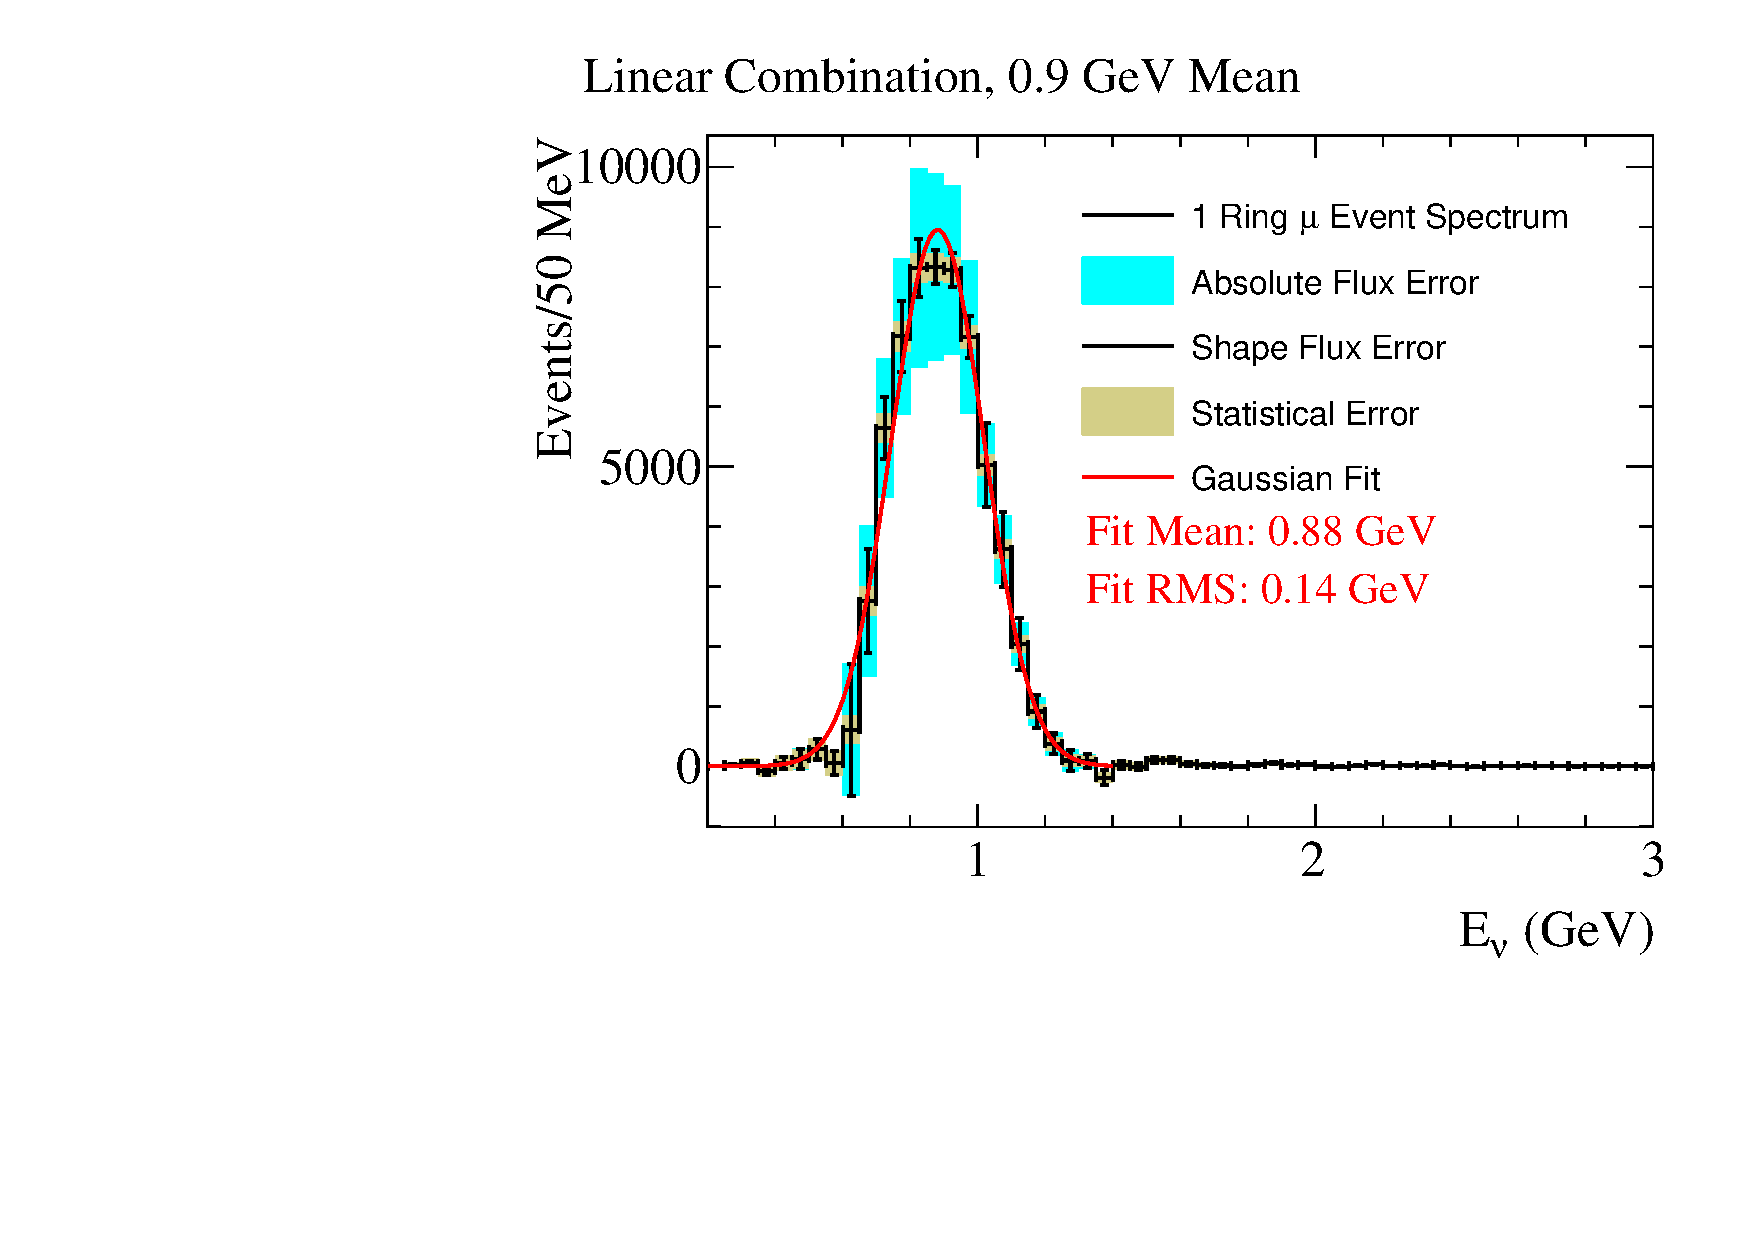
\includegraphics[width=0.45\textwidth]{figures/lc_etrue_900mev.pdf} \\
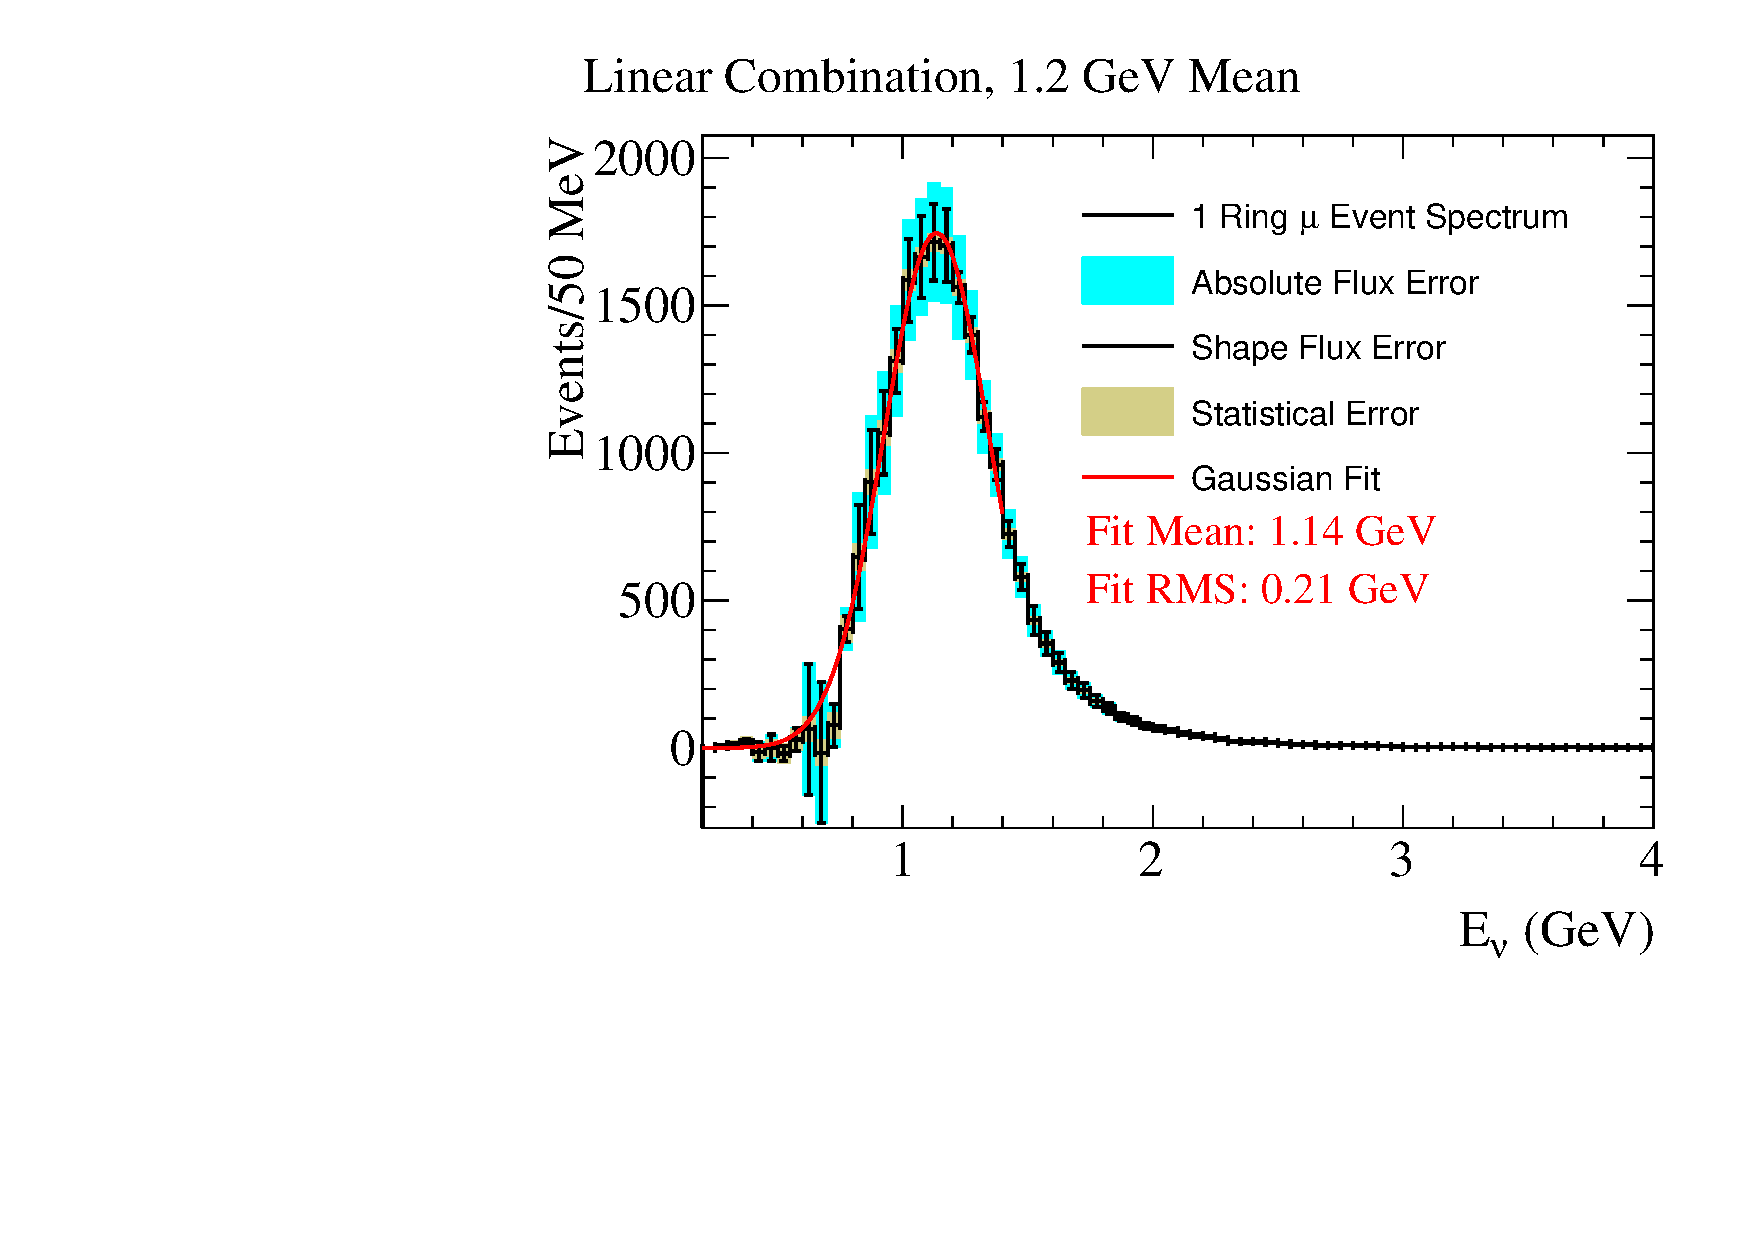
\includegraphics[width=0.45\textwidth]{figures/lc_etrue_1200mev.pdf} 
\caption{Three ``pseudo-monochromatic" spectra centered at 0.6 (top), 0.9 (middle) and 1.2 (bottom) GeV.  The aqua error bars show
the 1 $\sigma$ uncertainty for flux systematic variations, while the black error bars show the flux systematic variation after the
overall normalization uncertainty is removed.  The tan error bars show the statistical uncertainty for samples corresponding to 
 $4.5\times10^{20}$ protons on target.  }
\label{fig:mono_beam}
\end{figure}

%\begin{figure}[htpb]
%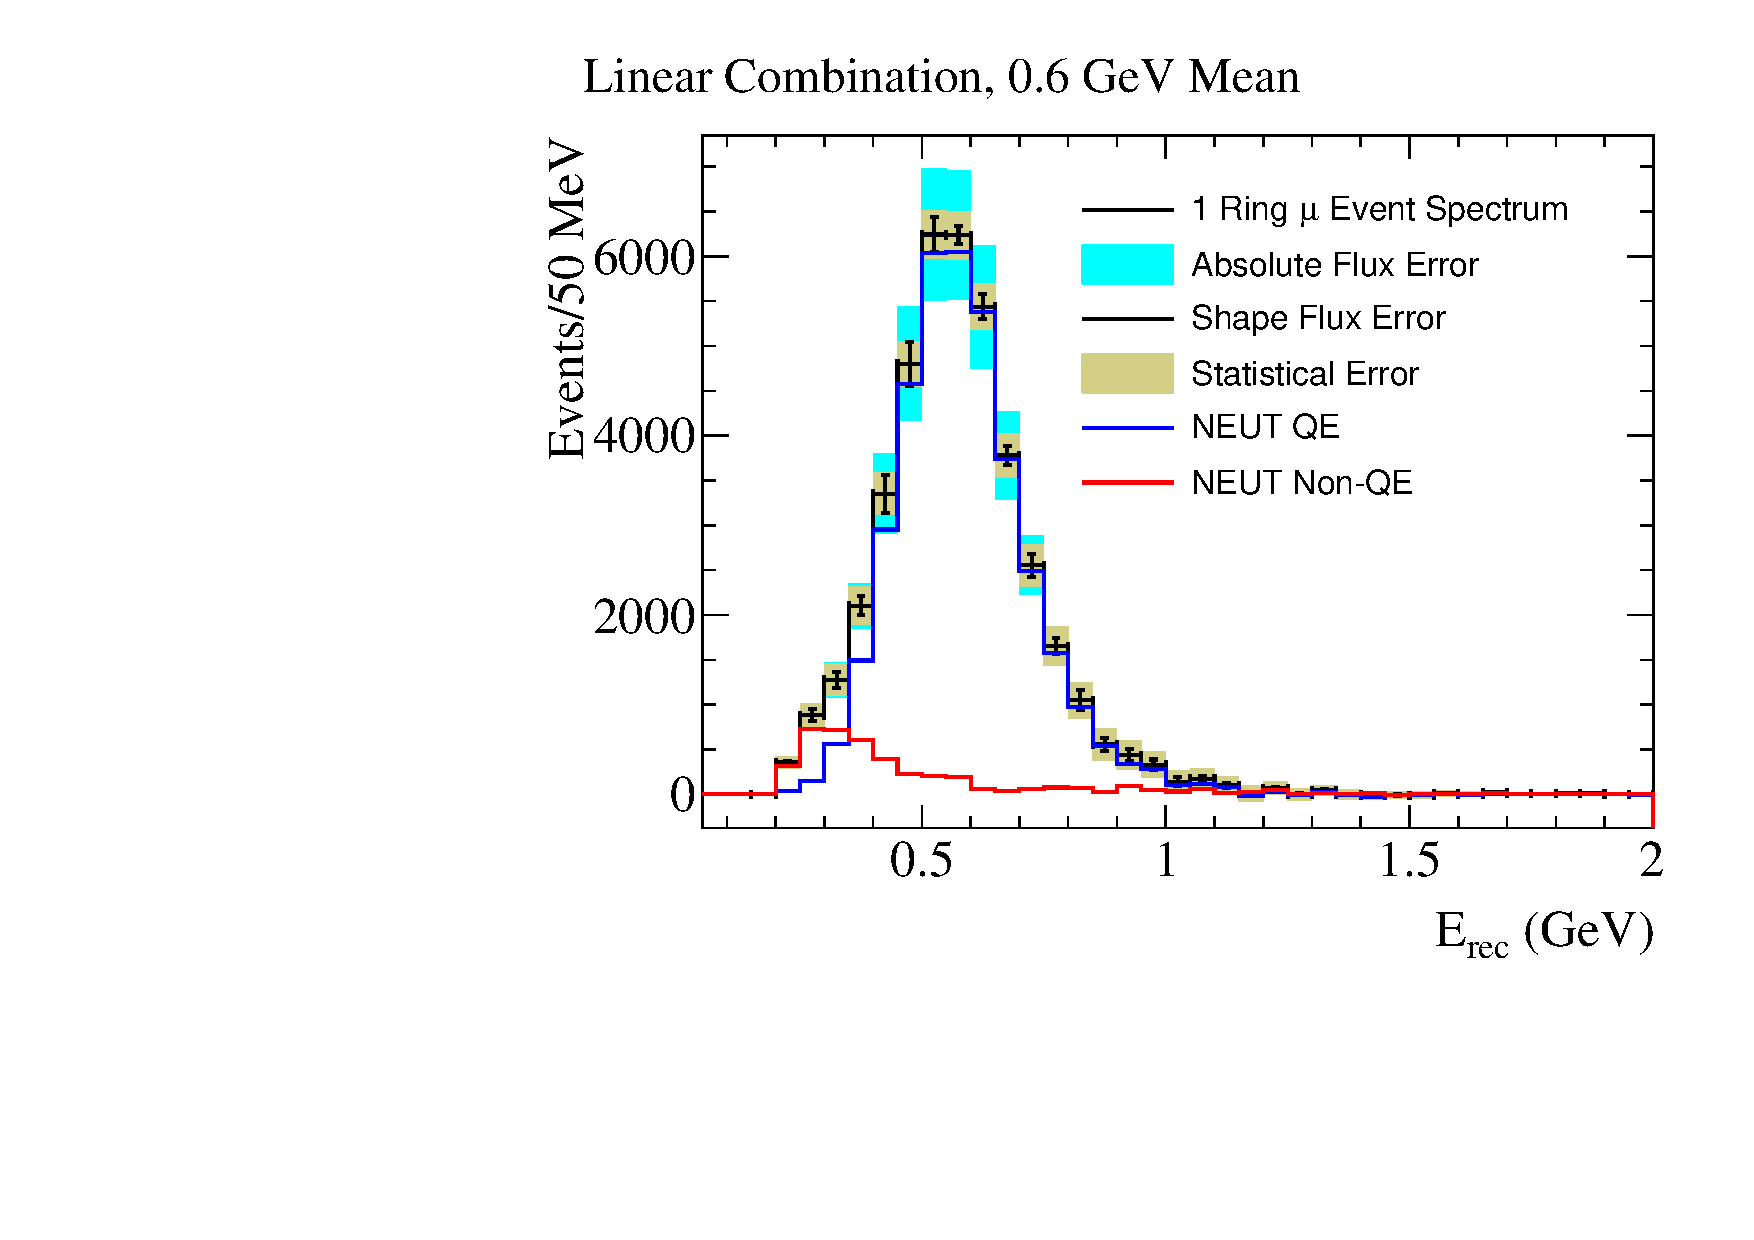
\includegraphics[width=0.45\textwidth]{figures/lc_erec_600mev.pdf} \\
%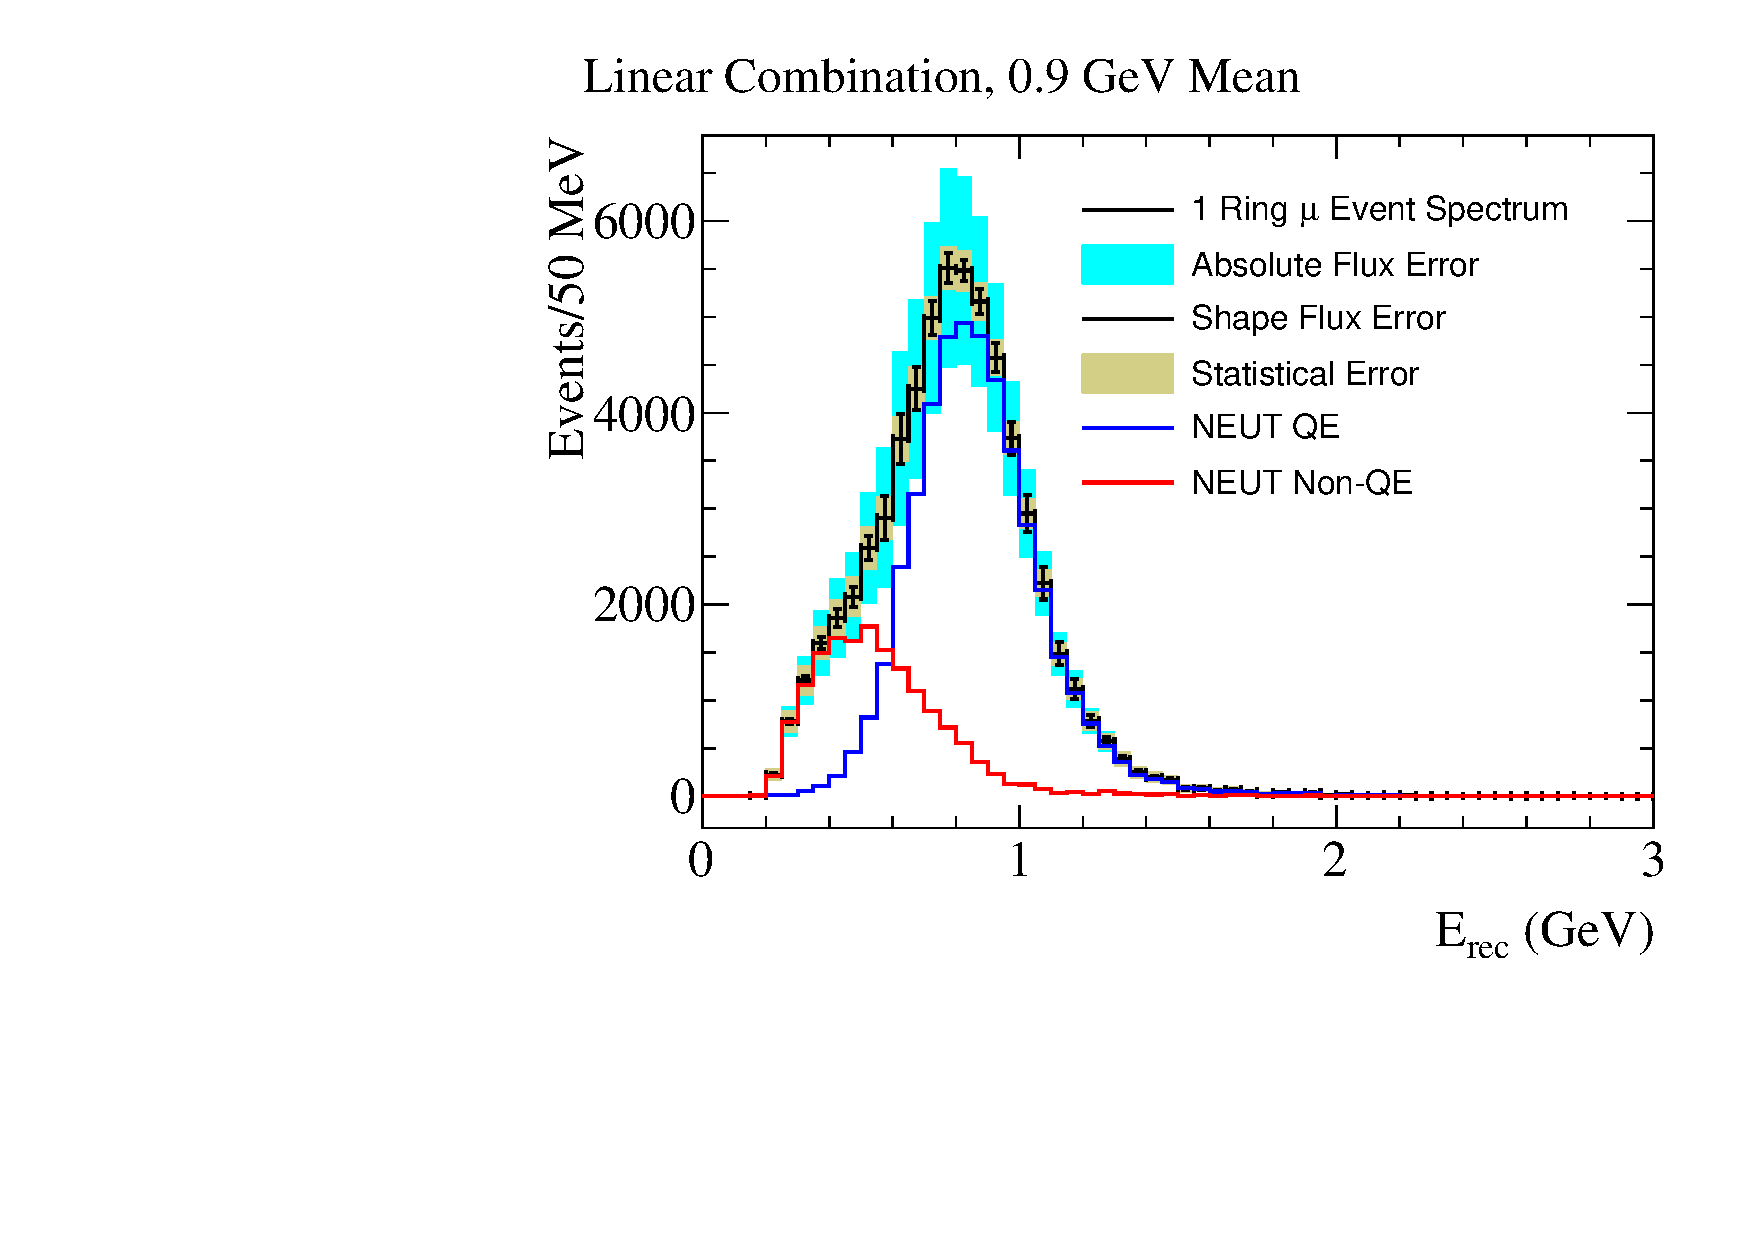
\includegraphics[width=0.45\textwidth]{figures/lc_erec_900mev.pdf} \\
%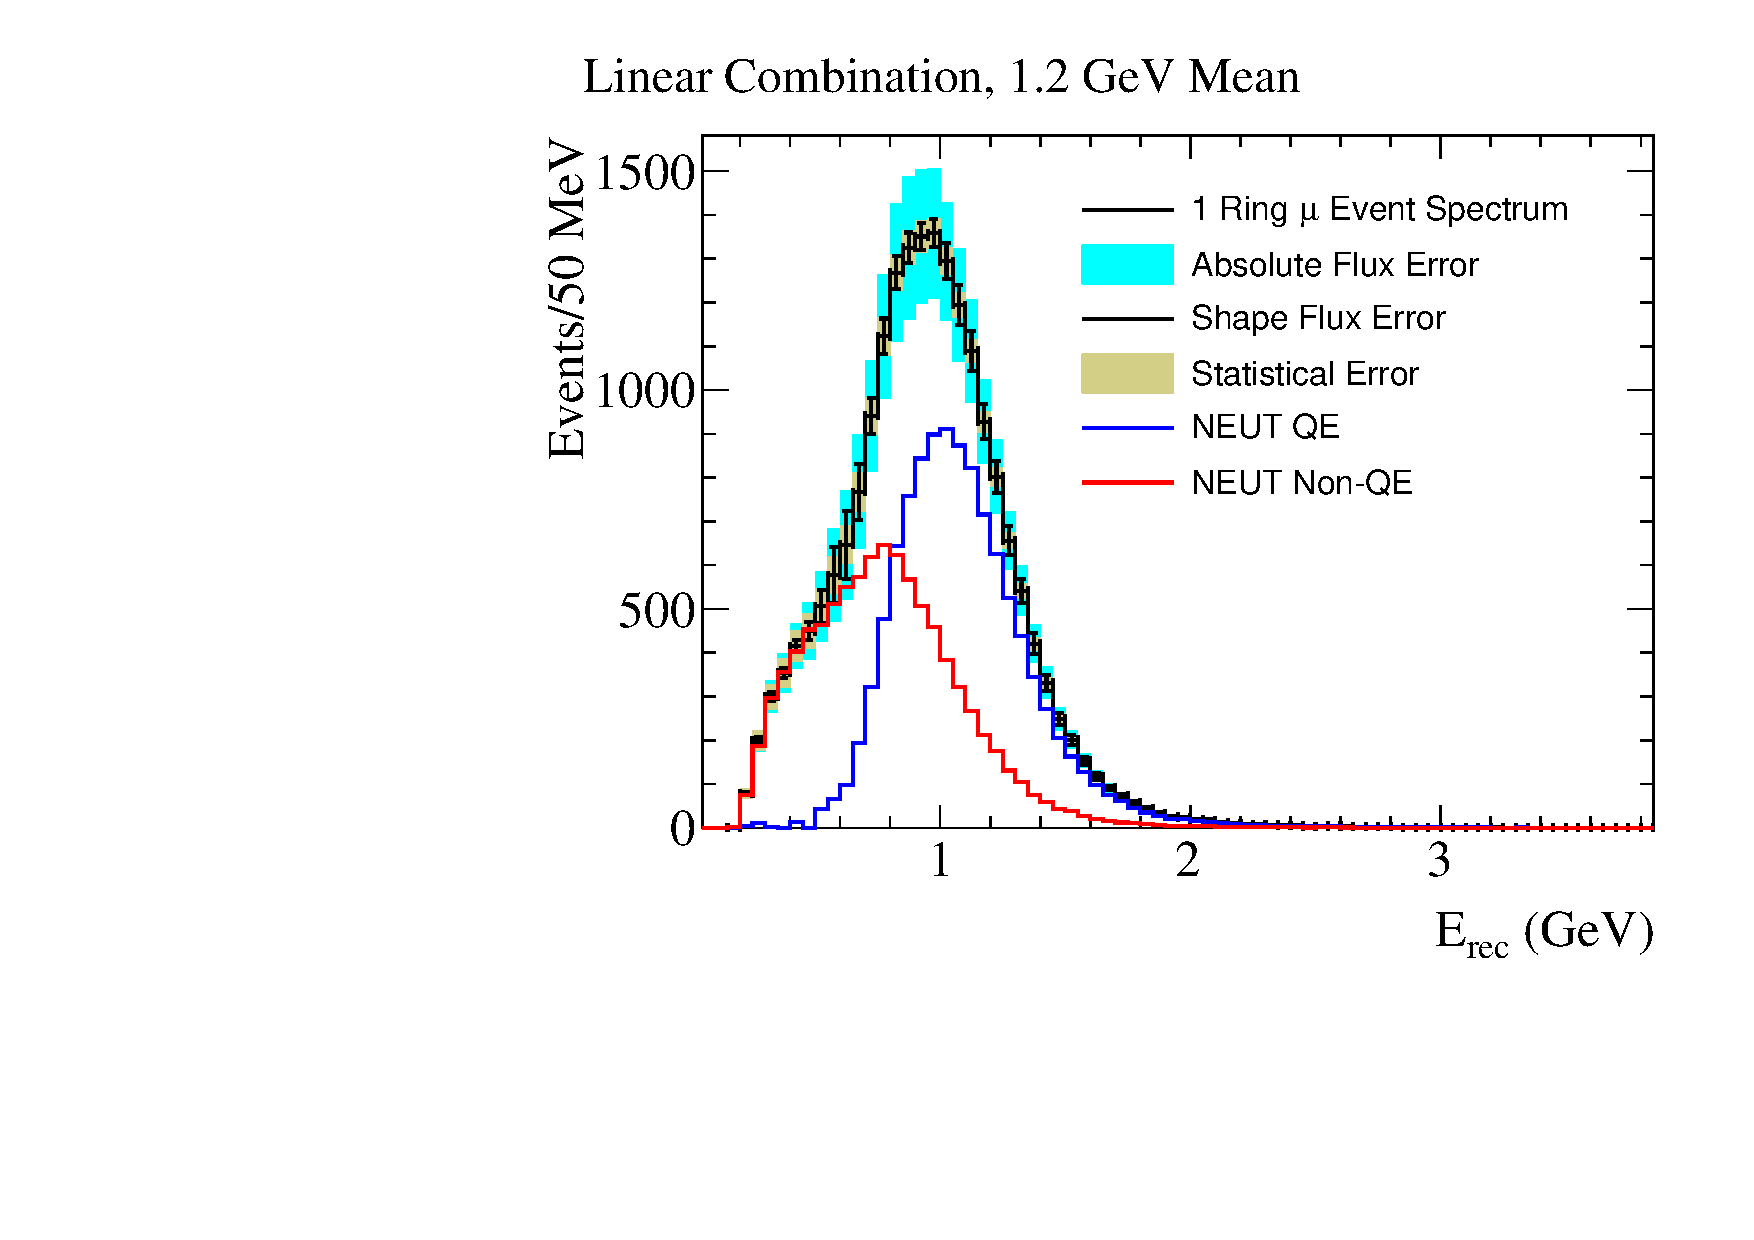
\includegraphics[width=0.45\textwidth]{figures/lc_erec_1200mev.pdf} 
%\caption{The reconstructed energy distributions for 1-ring muon candidate events produced using 
%``pseudo-monochromatic" spectra centered at 0.6 (top), 0.9 (middle) and 1.2 (bottom) GeV.  The aqua error bars show
%the 1 $\sigma$ uncertainty for flux systematic variations, while the black error bars show the flux systematic variation after the
%overall normalization uncertainty is removed.  The tan error bars show the statistical uncertainty for samples corresponding to 
% $4.5\times10^{20}$ protons on target.  The red and blue histograms show the contributions from non-quasi-elastic and quasi-elastic
%scatters respectively. }
%\label{fig:mono_beam_erec}
%\end{figure}

% example eA plots

%----


% measurements of CCQE, CC1pi+
%% reference what has been done historically. Current disagreement and resolution?  CC1pi+ disagreement in deuterium data, CCQE axial form factor -> MEC?, NC/CC. 
%Recent measurements of pion production by MiniBooNE is not explained without severe modifications to the final state interaction model. 
% nue/numu cross section ratio, mention in later section?

% CCQE measured by MiniBooNE, MINERvA, NOMAD, and SciBooNE.
% On water, measurement by K2K, tie to earlier section.

No consensus of the CCQE cross section has emerged from neutrino experiments on {12}^C and {16}^O targets. The K2K experiment reported a value of the axial mass, $M_A$ of $1.20 \pm 0.12$~GeV~\cite{Gran:2006jn} corresponding to an enhanced cross section relative to expectation. Similar results have been reported on carbon by MiniBooNE~\cite{AguilarArevalo:2010zc} and SciBooNE~\cite{sciboone-nuint2011}, and T2K~\cite{Abe:2014iza}. Figure~\ref{fig:ccqe} summarizes the reported CCQE cross section as a function of true neutrino energy, inferred from a single nucleon

%Nieves paper shows this assumption can cause issues
% nuclear effects too.


 In addition, a measurement by NOMAD~\cite{Lyubushkin:2008pe} was done at higher neutrino energies which is not in agreement with MiniBooNE and SciBooNE. This is shown in Figure~\ref{fig:ccqe}, along with the recent T2K ND280 Tracker analysis results. An indirect measurement of the cross section was done with the K2K near detectors, where a higher than expected value of the QE axial mass, $M_A$, was also reported~\cite{Gran:2006jn}. There are also recent results from MINERvA~\cite{Fiorentini:2013ezn}.

\begin{figure}[htpb]
\begin{center}
      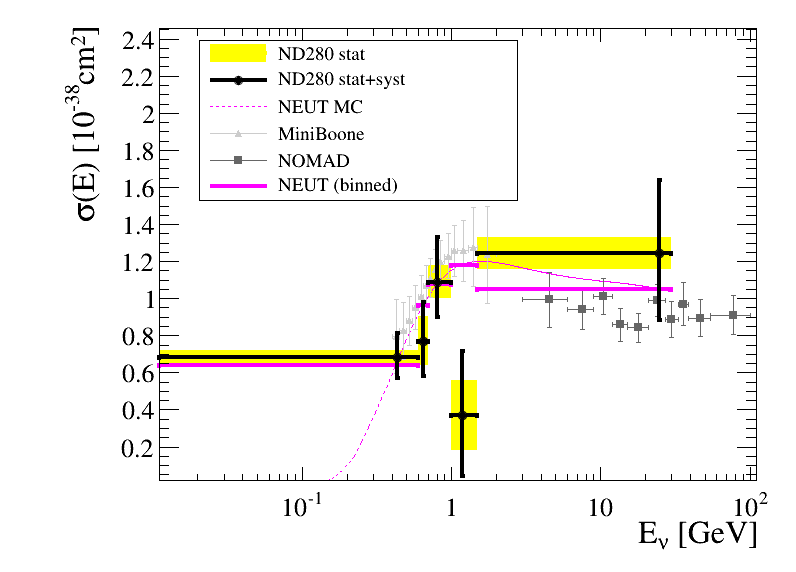
\includegraphics[width=0.45\textwidth] {figures/nd280_miniboone_nomad.png}
\end{center}
\caption{The CCQE cross section as predicted by NEUT (pink dashed) vs. true neutrino energy. Also overlaid are results from MiniBooNE, NOMAD and T2K.}
\label{fig:ccqe}
\end{figure}


MiniBooNE's selection was CC0$\pi$, that is 1 muon and no pions in the final state, and was 77.0\% pure and 26.6\% efficient; the \rmu selection at SK is 91.7\% pure  and 93.2\% efficient, based on observable final state.
It is postulated that the MiniBooNE selection, but not the NOMAD one, is sensitive to multinucleon processes, where a neutrino interacts on a correlated pair of nucleons and that this resulted in the higher cross section reported by MiniBooNE. However, the two experiments have very different flux, selection and background predictions and systematics.

By measuring the CC0$\pi$ cross section  at different vertex points in \nuprismlite, we should be able to infer the different energy dependence and constrain multinucleon and CC1\pip pionless $\Delta$ decay (PDD)  processes. This can be seen in Figure~\ref{fig:mono_beam_erec}, which shows the momentum of CCQE and MEC (Nieves' npnh) events for a particular angular range ($0.85<$cos($\theta$)$<0.90$) generated according to the T2K flux, and for a 1~GeV \nuprismlite flux. MiniBooNE and T2K have difficulty separating the MEC component of the CCQE cross section due to the shape of their neutrino energy spectra, but the \nuprismlite detector would give us additional information to separate out that component and characterize it, as demonstrated in Figure~\ref{fig:mono_beam_erec}.  Even though \nuprismlite is not a measurement on carbon, oxygen is of a similar density to carbon and so will be helpful in understanding the difference between the MiniBooNE and NOMAD results if it is indeed due to MEC.

%\begin{figure}[h!]
%\begin{center}
%  \begin{minipage}[t]{.45\textwidth}
%    \begin{center}
%      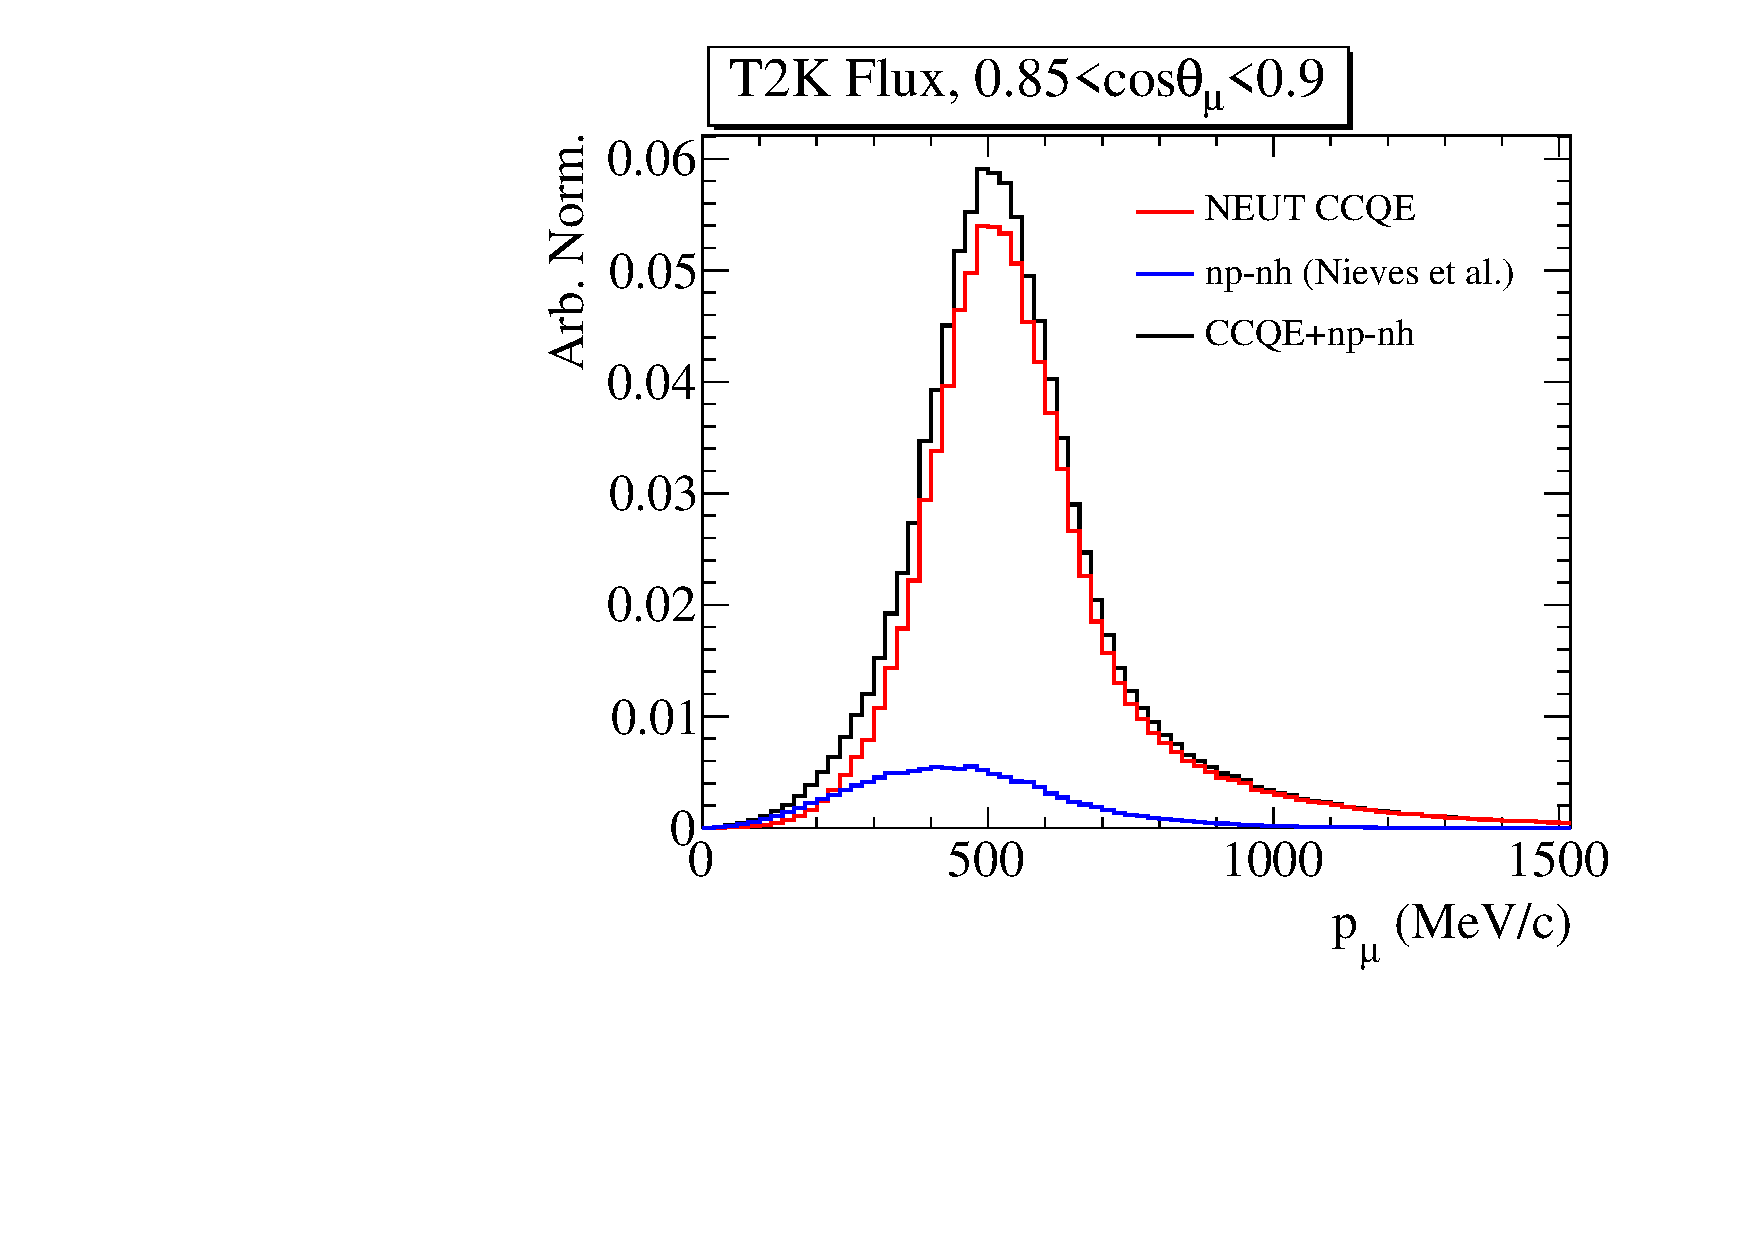
\includegraphics[width=\textwidth] {figures/t2kflux_ccqe_npnh.pdf}
%    \end{center}
%  \end{minipage}
%  \begin{minipage}[t]{.45\textwidth}
%    \begin{center}
%      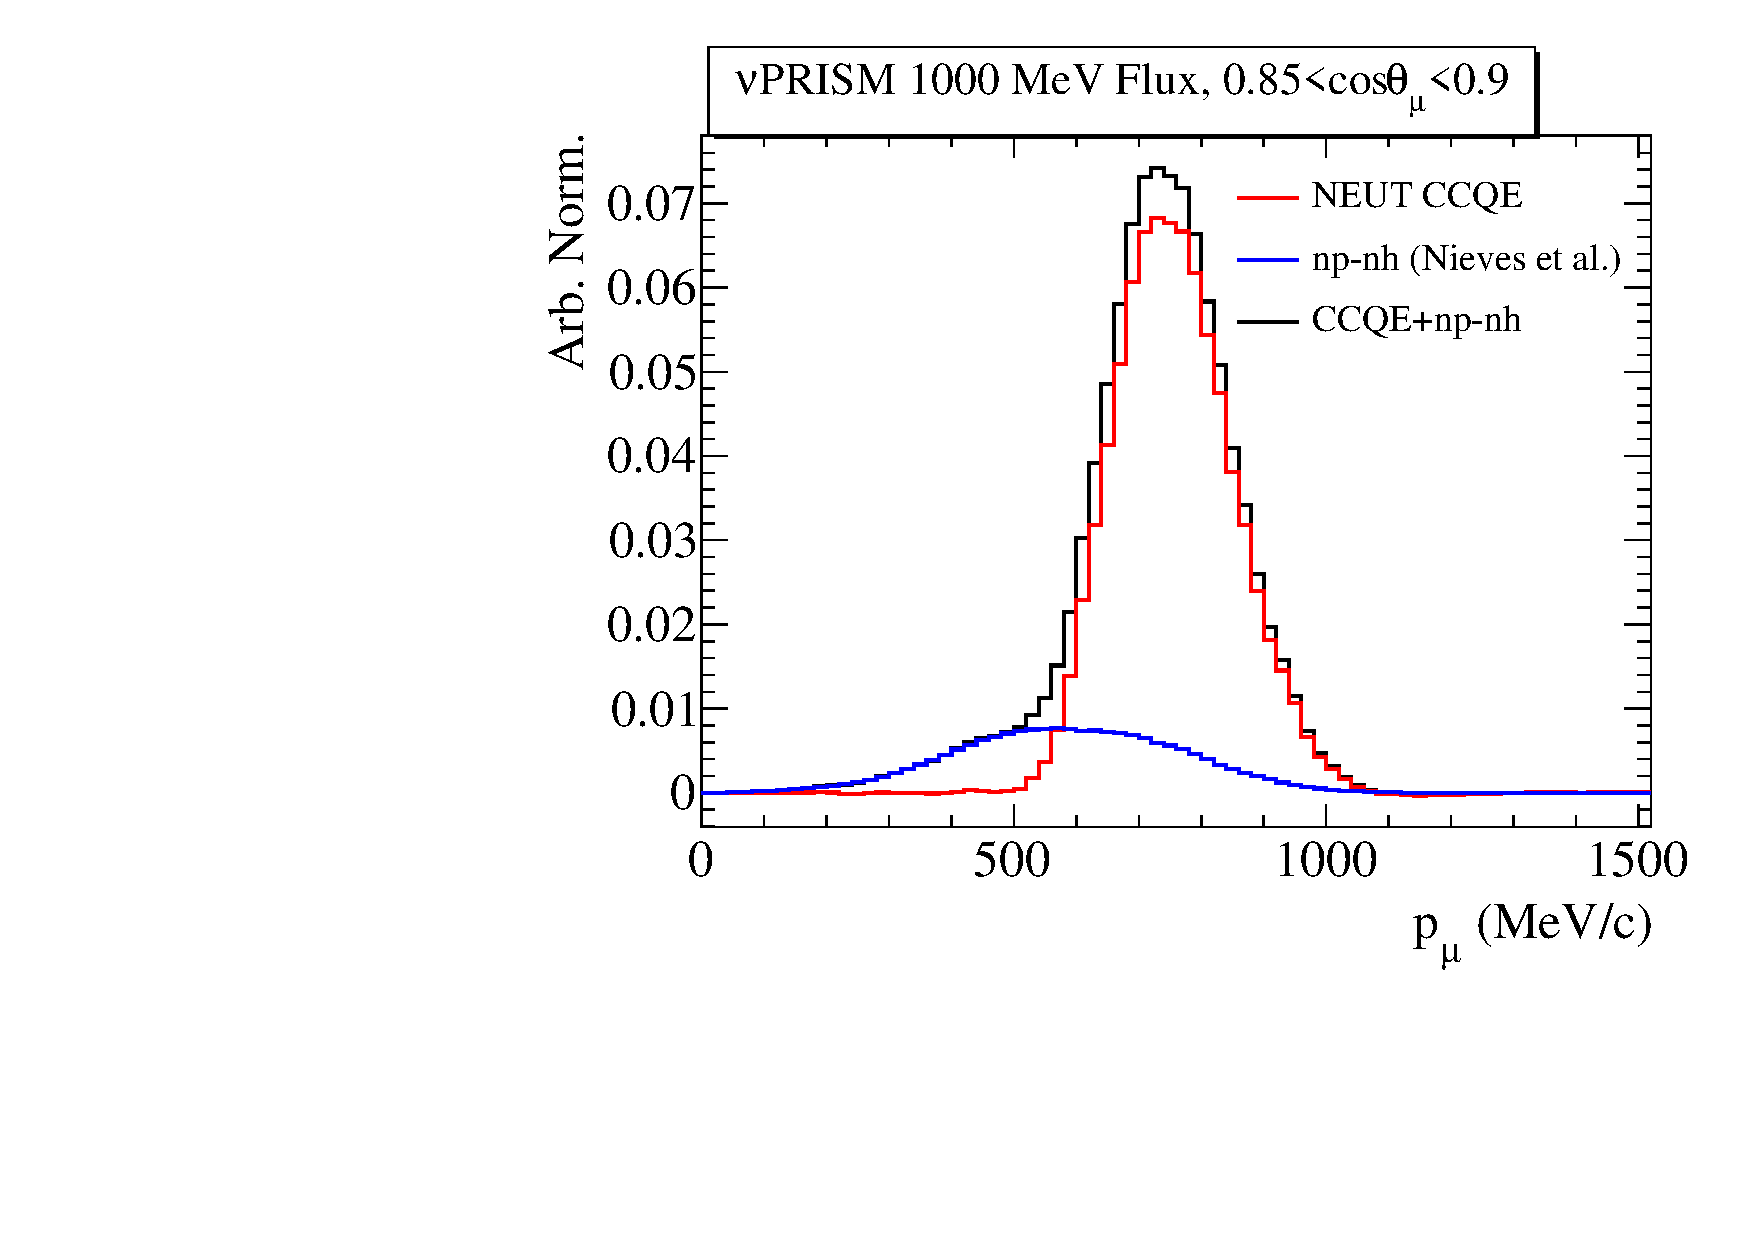
\includegraphics[width=\textwidth] {figures/nuprism1000flux_ccqe_npnh.pdf}
%    \end{center}
%  \end{minipage}
%\end{center}
%\caption{The momentum of CCQE and MEC (Nieves' npnh) events for a particular angular range ($0.85<$cos($\theta$)$<0.90$) generated according to the T2K flux (left), and for a 1000 MeV \nuprismlite flux (right)}
%\label{fig:npnh}
%\end{figure}

\subsubsection{CC1\pip and CC1\piz}

The CC1\pip and CC1\piz cross sections have been measured on carbon by MiniBooNE~\cite{AguilarArevalo:2010bm},\cite{AguilarArevalo:2010xt}; K2K also produced measurements CC1\pip~\cite{Rodriguez:2008aa} and CC1\piz~\cite{Mariani:2010ez} with the SciBar detector. One may infer the coherent contribution to the CC1$\pi$ cross section from the angular distribution of the pion; this was done by K2K~\cite{Hasegawa:2005td} and SciBooNE. Improvements to the SK reconstruction could yield a similar efficiency and purity to the the MiniBooNE selections for CC1\pip (12.7\%, 90.0\%) and CC1\piz (6.4\%, 57.0\%) based on observable final state.

The CC1$\pi$ resonant cross section for the T2K flux is dominated by contributions from the $\Delta$ resonance~\cite{Lalakulich:2013iaa}, so \nuprismlite would provide clear information about the N$\Delta$ coupling and form factors. We can also compare the pion momentum produced out of CC1\pip interactions for different neutrino energies in order to better understand how final state interactions affect pion kinematics.

%{\it TODO: Add a plot of pion spectrum vs. offaxis angle} 


\subsubsection{NC1\pip and \ncpi}


In the current disappearance analysis, there are also substantial uncertainties on NC1$\pi^+$ and NC1$\pi^0$ processes (for disappearance and appearance respectively). As a result, future proposed experiments which use water as a target (e.g. Hyper-Kamiokande and CHIPS) will directly benefit from the \nuprismlite cross section program; other programs benefit less directly through a critical validation of our assumptions of the energy dependence of the cross section on oxygen.
 Furthermore, there is no data for the kinematic information of pions out of NC\pip interactions. However, NC\pip is one of the backgrounds in the current T2K \rmu selection used for the disappearance analysis. A direct measurement of NC\pip, and a measurement of the pion momentum and angular distributions would reduce the substantial uncertainties on this process (in both cross section and detector efficiency) in the analysis.


The \ncpi  cross section has been measured on carbon by MiniBooNE~\cite{AguilarArevalo:2009ww} (36\% efficient, 73\% pure) and SciBooNE. A measurement of the ratio of \ncpi to the CCQE cross section has been done water by the K2K 1kton near detector~\cite{Nakayama:2004dp}. The efficiency and purity of the K2K selection is 47\% and 71\% respectively. A measurement of NC\pip exists~\cite{hawker} on a complicated target material (C$_3$H$_8$CF$_3$Br) but has no differential kinematic information. Figure~\ref{fig:ncpip} shows this measurement with a prediction from the NUANCE neutrino event generator.  

\begin{figure}[htpb]
\begin{center}
      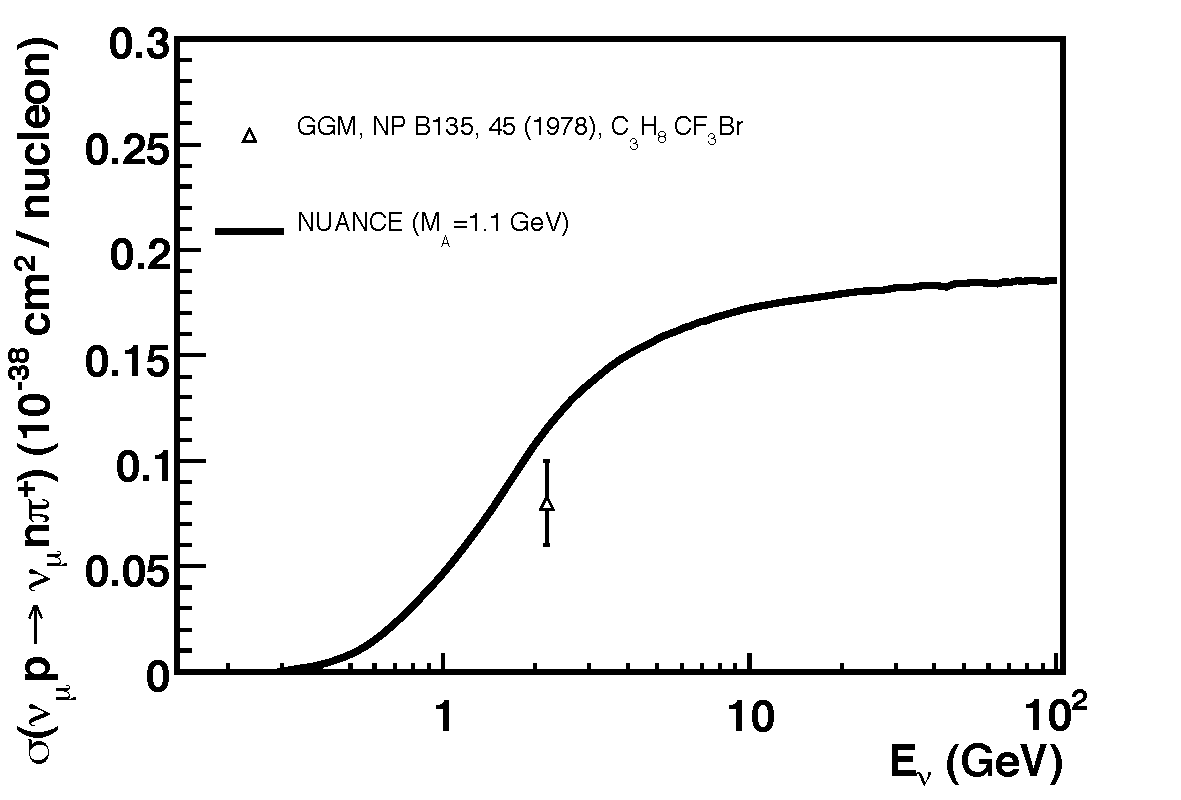
\includegraphics[width=0.45\textwidth] {figures/plot_ncpip_nu.pdf}
\end{center}
\caption{The NC\pip  cross section as predicted by NUANCE vs. true neutrino energy overlaid with the only measurement (on C$_3$H$_8$CF$_3$Br). Figure from Ref.~\cite{Formaggio:2013kya}}
\label{fig:ncpip}
\end{figure}

A measurement of NC\pip will be challenging but possible at \nuprismlite. T2K already has developed an ``NC'' enhanced selection for Super-K that is 24\% NC\pip, 14\% NC1proton, and 55\% CC\numu, by interaction mode. Recent developments in event reconstruction at Super-K include a dedicated pion ring finder, which should make possible a more pure selection of NC\pip from which the pion momentum and angular distribution can also be measured. Since \nuprismlite will allow for a first measurement of the energy dependence of the NC channels and like the CC channels, it will be particularly interesting to measure the outgoing pion spectra of these events in order to probe nuclear final state interactions.


% Unique measurements of NC processes.
%% Lack of information about NCpi+, NC1gamma. List of processes expected based on historic measurements **refs 1kton


